\documentclass{article}

\usepackage[dutch]{babel}
\usepackage[margin=3cm]{geometry}
\usepackage{graphicx}
\usepackage{float}
\usepackage{caption}
\usepackage{hyperref}
\usepackage{amsmath}
\usepackage{wrapfig}
\usepackage[parfill]{parskip}

% fonts
\usepackage[T1]{fontenc}
\usepackage{helvet}
\renewcommand{\familydefault}{\sfdefault}

\graphicspath{{img/}}

% theorem environment
\usepackage{amssymb}

\newtheorem{theorem}{Definitie}[section]

\usepackage{enumitem}

\newenvironment{thmenum}
 {\begin{enumerate}[label=\upshape\bfseries(\roman*)]}
 {\end{enumerate}}


% code
\usepackage{minted}
\usepackage{upquote}
\usepackage{color}

\begin{document}

\begin{titlepage}
    \author{Tuur Vanhoutte}
    \title{Machine Learning \& AI}
\end{titlepage}

\pagenumbering{gobble}
\maketitle
\newpage
\tableofcontents
\newpage

\pagenumbering{arabic}

\section{Inleiding}

\subsection{AI in context}

\begin{figure}[H]
    \centering
    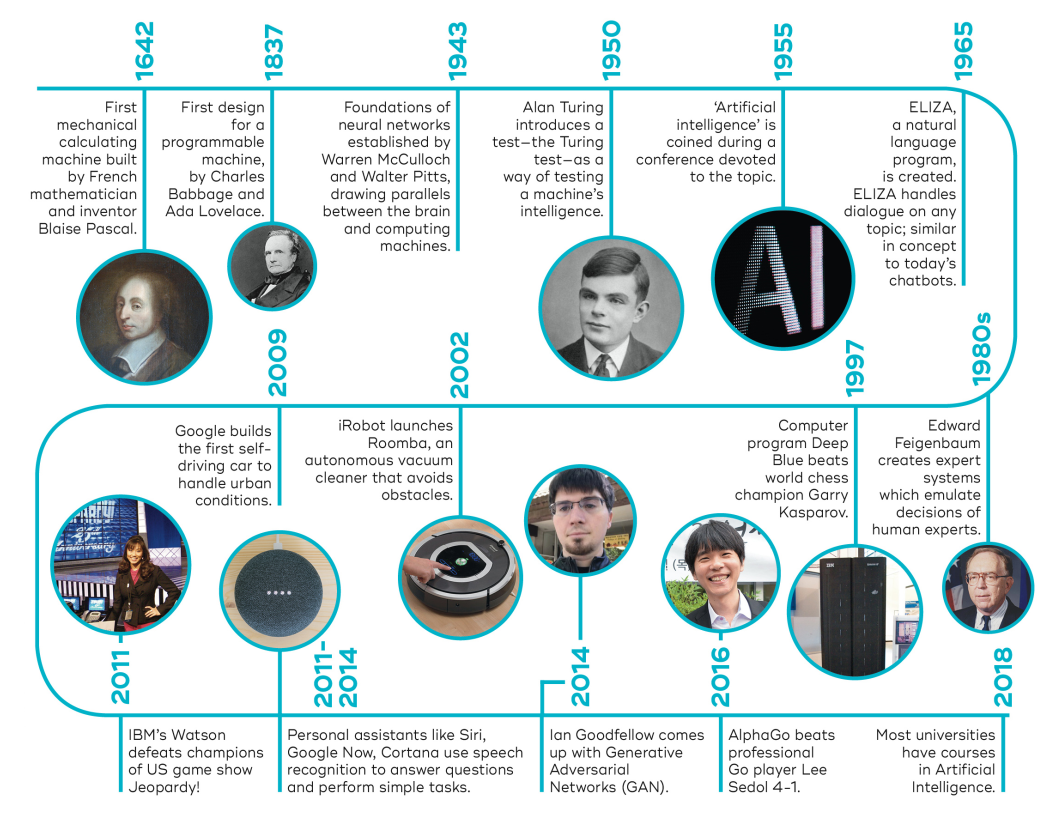
\includegraphics[width=0.5\textwidth]{ai-history.png}
    \caption{Geschiedenis van AI}
\end{figure}

Belangrijkste gebeurtenissen:

\begin{itemize}
    \item \textbf{1943:} McCulloch - Pitts: fundering van neurale netwerken
    \item \textbf{1950:} Alan Turing: de Turing test
    \item \textbf{1956:} Dartmouth workshop: bijeenkomst voor breinstorm AI
    \item \textbf{1997:} Garry Kasparov vs Deep Blue (IBM)
    \item \textbf{2011:} IBM Watson
    \item \textbf{2016:} AlphaGo
    \item \textbf{2021-:} toekomst
\end{itemize}

\subsubsection{Vormen van AI}

\begin{itemize}
    \item Zwakke AI (weak AI / Artificial Narrow Intelligence)
    \begin{itemize}
        \item Goed in een bepaalde taak maar alleen in die taak
        \item \textbf{Voorbeelden: } spamfilters, schaakcomputers, gezichtsherkenning
    \end{itemize}
    \item Sterke AI (strong AI / Artificial General Intelligence)
    \begin{itemize}
        \item Intelligentie op menselijk niveau
        \item In staat om zich aan te passen en problemen te leren oplossen in verschillende contexten
    \end{itemize}
    \item Superintelligentie (Artificial Super Intelligence)
    \begin{itemize}
        \item Als AI zelfbewust wordt en de mens op alle vlakken voorbij steekt
    \end{itemize}
\end{itemize}

\begin{figure}[H]
    \centering
    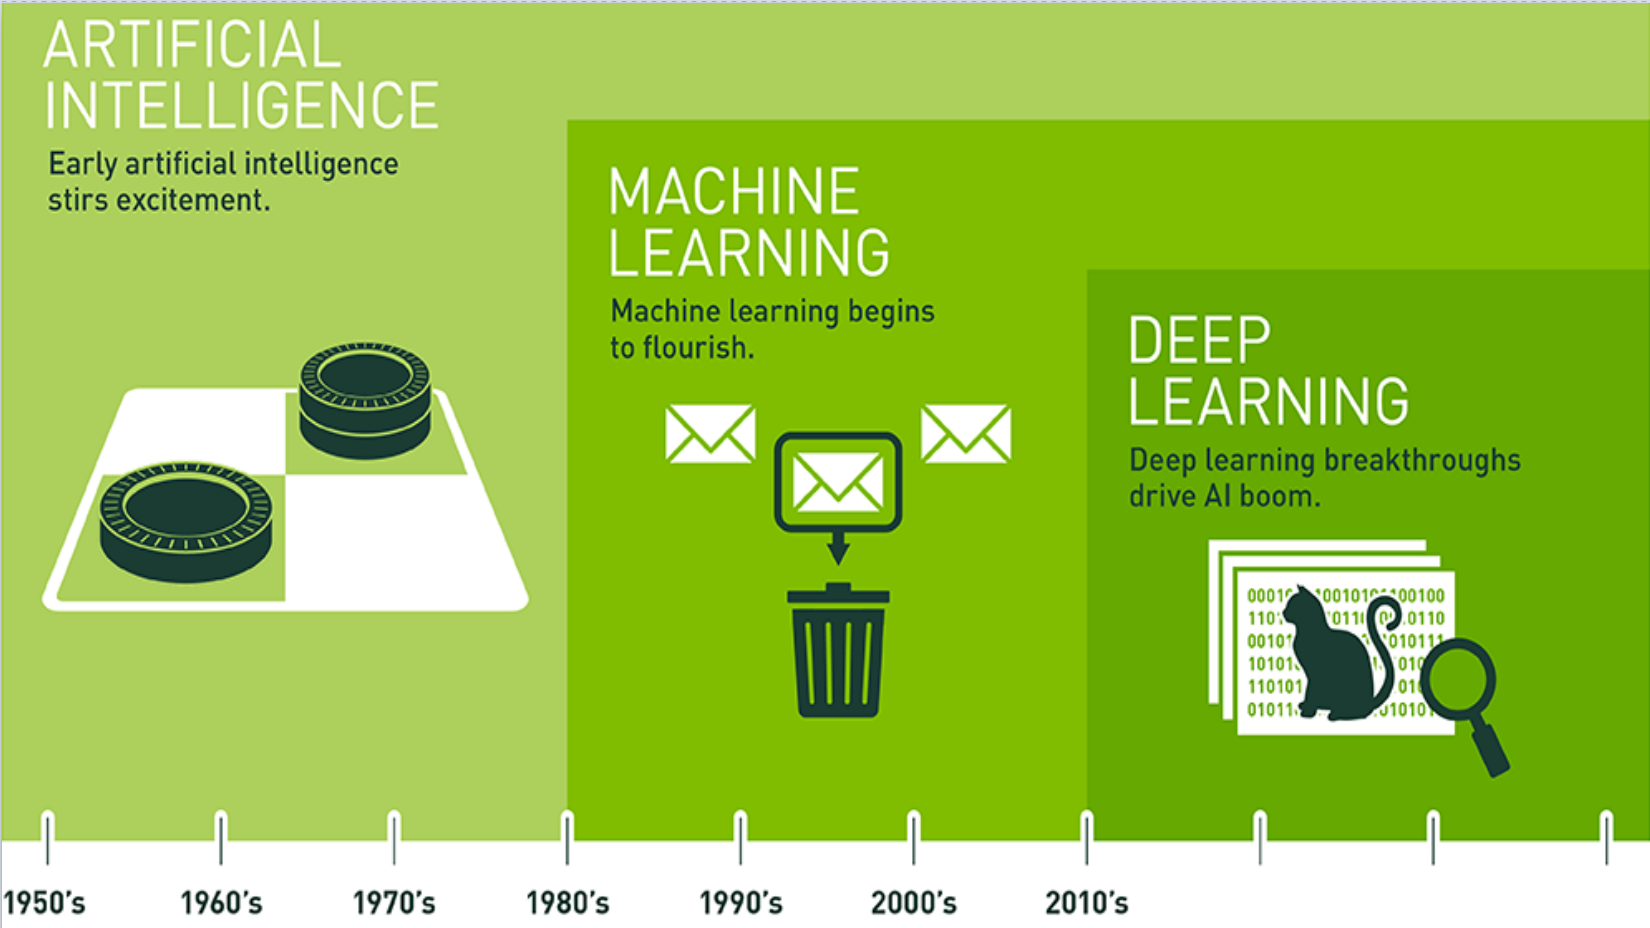
\includegraphics[width=0.6\textwidth]{ai-history2.png}
    \caption{AI vs ML vs DL}
\end{figure}

\subsubsection{Sectoren die de planeet verbeteren}

\begin{itemize}
    \item Klimaatsverandering
    \item Biodiversiteit en conservatie
    \item Water
    \item Hernieuwbare energie
    \item Medische sector
    \item Weer- en rampenvoorspelling
\end{itemize}

\subsubsection{Waarom nu?}

\begin{itemize}
    \item Snellere hardware
    \item Betere algoritmes
    \item Meer data
    \item (Open source) frameworks
\end{itemize}

\begin{figure}[H]
    \centering
    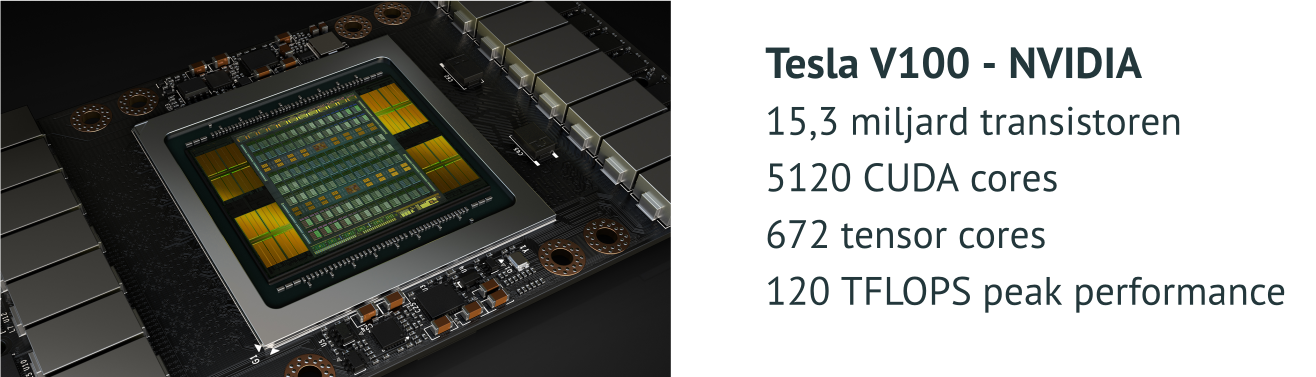
\includegraphics[width=0.5\textwidth]{nvidia-tesla.png}
    \caption{Voorbeeld huidige hardware: de Tesla V100 van Nvidia}
\end{figure}

\section{Hoe leren uit data?}

\subsection{Leeralgoritmes}

\begin{itemize}
    \item Supervised
    \begin{itemize}
        \item Inputs met gewenste outputs zijn gegeven
        \item Task driven
    \end{itemize}
    \item Unsupervised
    \begin{itemize}
        \item De gewenste outputs zijn niet gegeven
        \item Data driven (clustering)
    \end{itemize}
    \item Reinforcement
    \begin{itemize}
        \item Beslissingsproces op basis van beloningen
        \item Algoritme leert te reageren op zijn omgeving
    \end{itemize}
\end{itemize}

\begin{figure}[H]
    \centering
    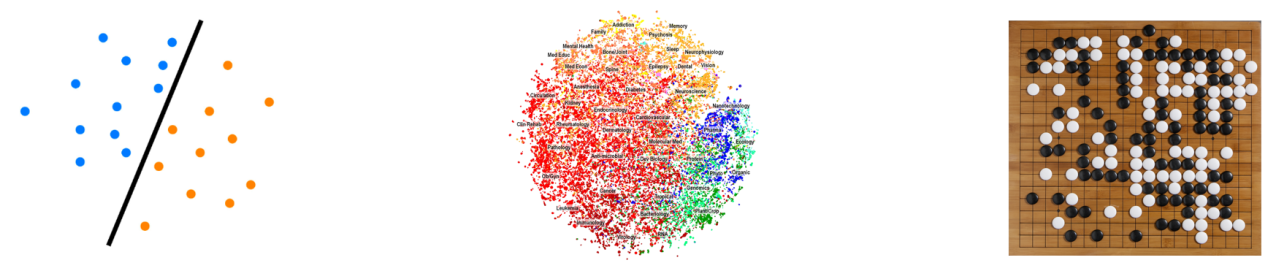
\includegraphics[width=0.5\textwidth]{leeralgoritmes.png}
    \caption{Supervised / Unsupervised / Reinforcement learning}
\end{figure}


\subsection{Supervised Learning}

Leren uit een gelabelde dataset. Vind het verband tussen de features en de labels

\begin{figure}[H]
    \centering
    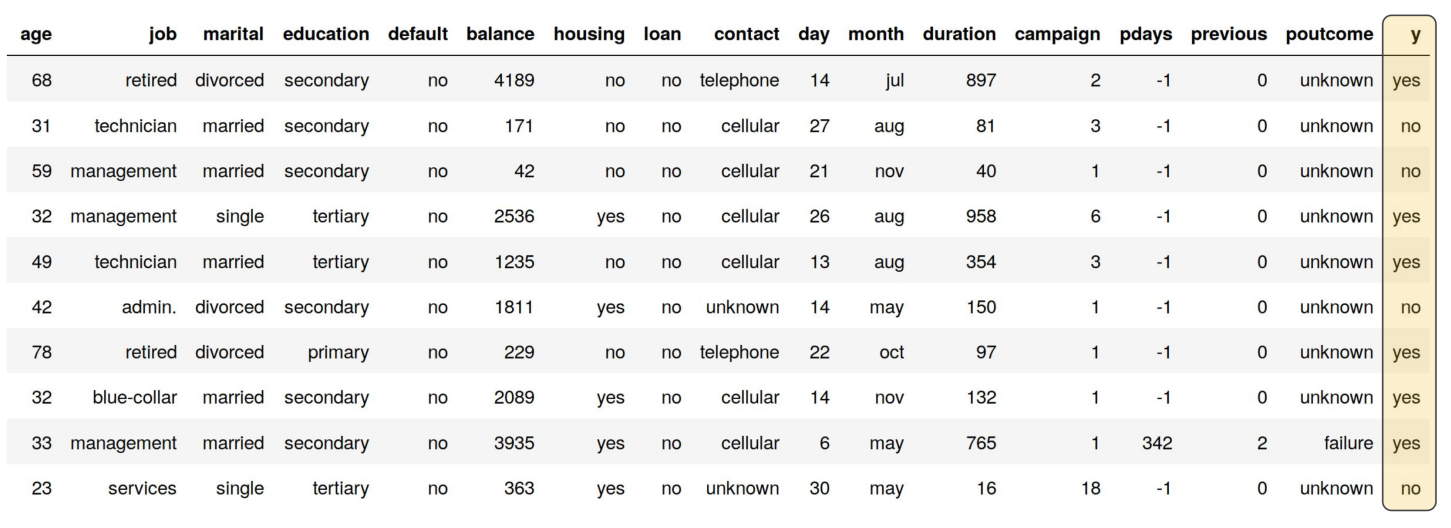
\includegraphics[width=0.5\textwidth]{supervised-learning.png}
    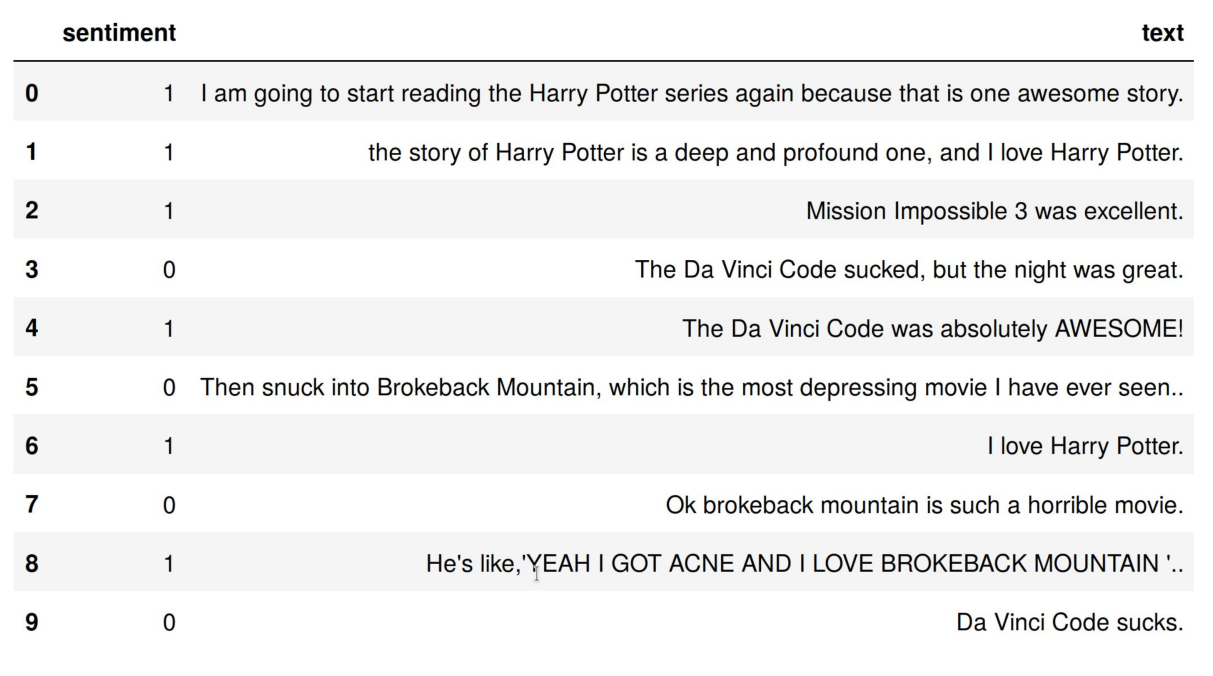
\includegraphics[width=0.4\textwidth]{supervised-learning2.png}
    \caption{Leren uit een dataset}
\end{figure}

\begin{figure}[H]
    \centering
    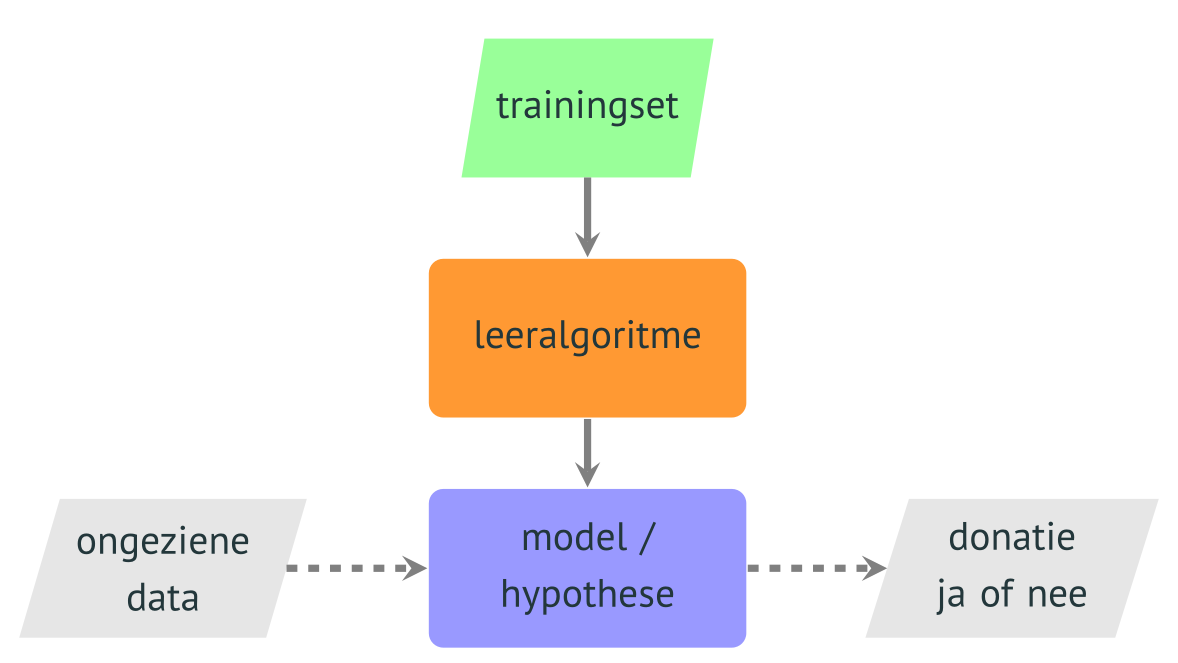
\includegraphics[width=0.5\textwidth]{supervised-learning3.png}
    \caption{Supervised learning kan uit ongeziene data een resultaat berekenen}
\end{figure}

\subsubsection{Regressie vs Classificatie}

\begin{figure}[H]
    \centering
    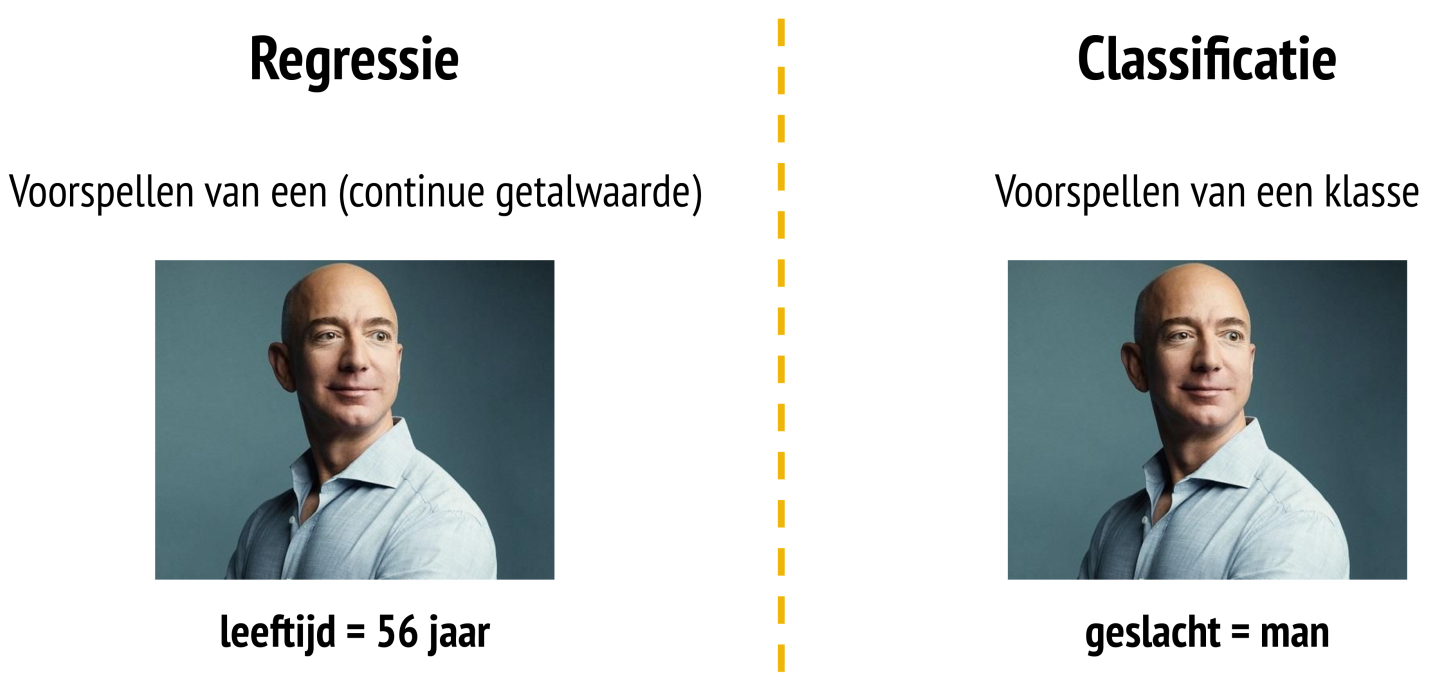
\includegraphics[width=0.5\textwidth]{regressie-vs-classificatie.png}
    \caption{Regressie vs classificatie}
\end{figure}

\begin{figure}[H]
    \centering
    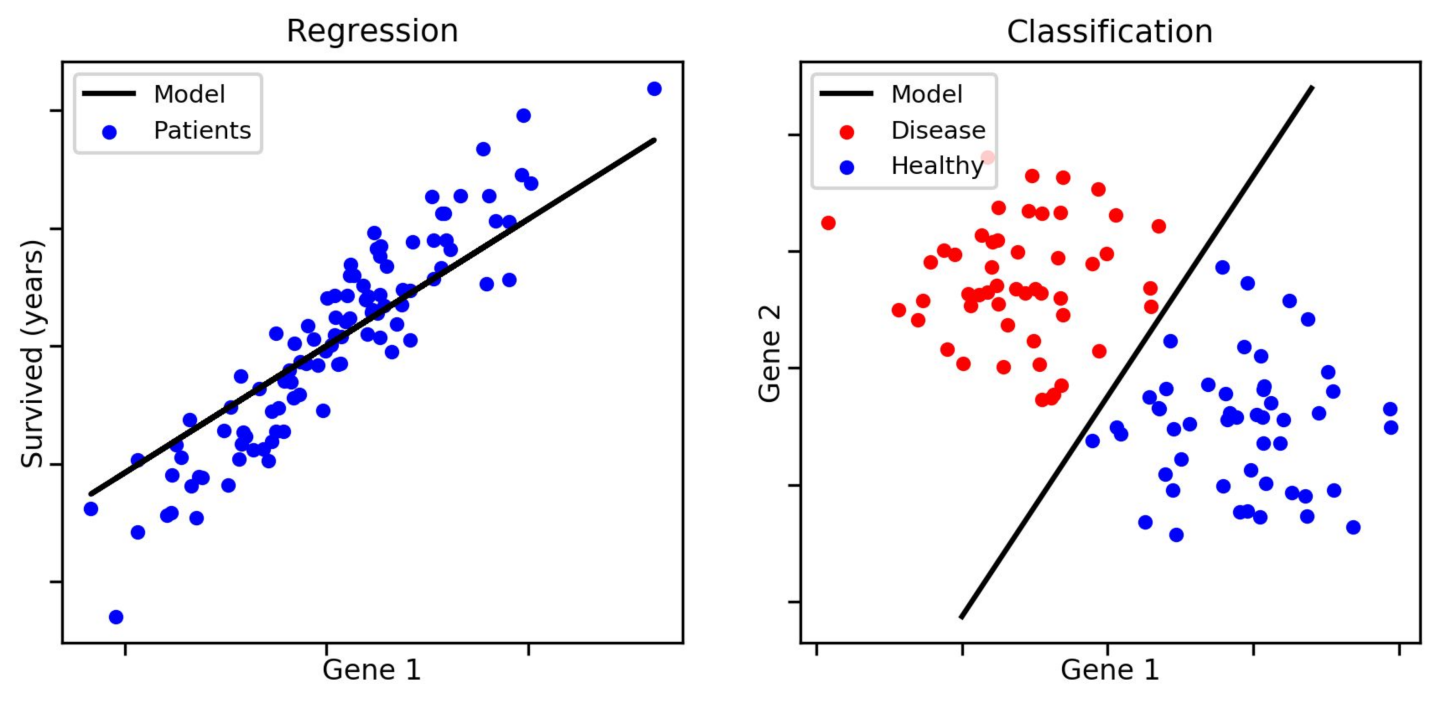
\includegraphics[width=0.5\textwidth]{regressie-vs-classificatie2.png}
    \caption{Regressie vs classificatie}
\end{figure}

\subsubsection{Voorbeeld}

Hoe stuurhoek bepalen bij een self-driving car?

\begin{itemize}
    \item (infrarood) camera's
    \item Stereo vision
    \item Radar
    \item LIDAR
    \item GPS
    \item Audio
\end{itemize}

\begin{figure}[H]
    \centering
    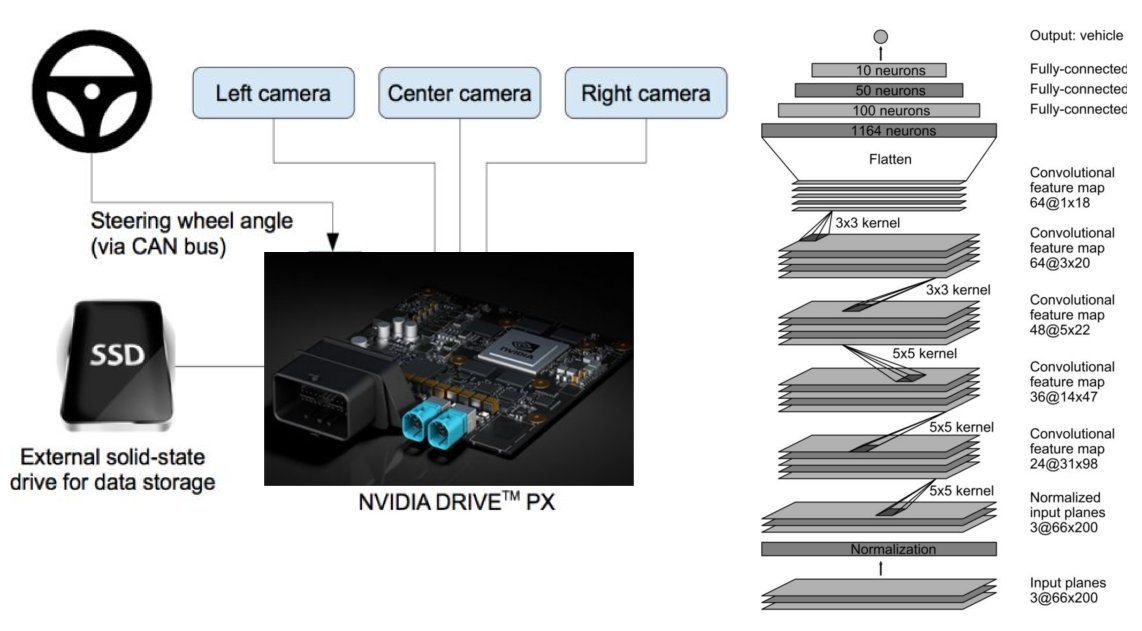
\includegraphics[width=0.6\textwidth]{stuurhoek-selfdriving-car.png}
    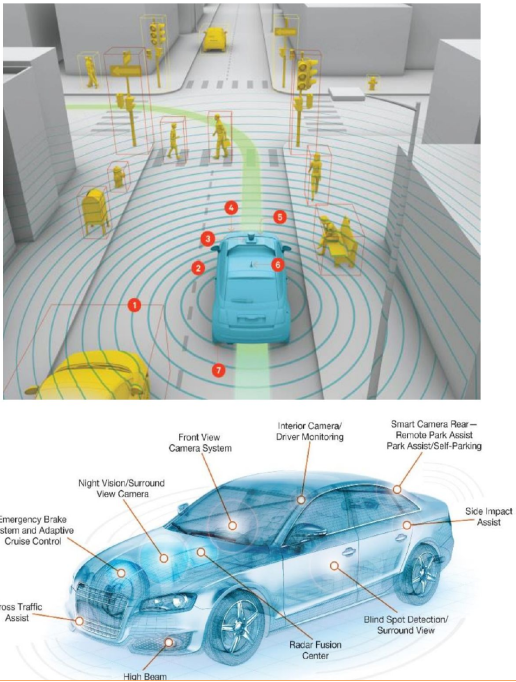
\includegraphics[width=0.3\textwidth]{stuurhoek-selfdriving-car2.png}
    \caption{Via sensoren weet de auto }
\end{figure}



\subsection{Unsupervised learning}

\begin{figure}[H]
    \centering
    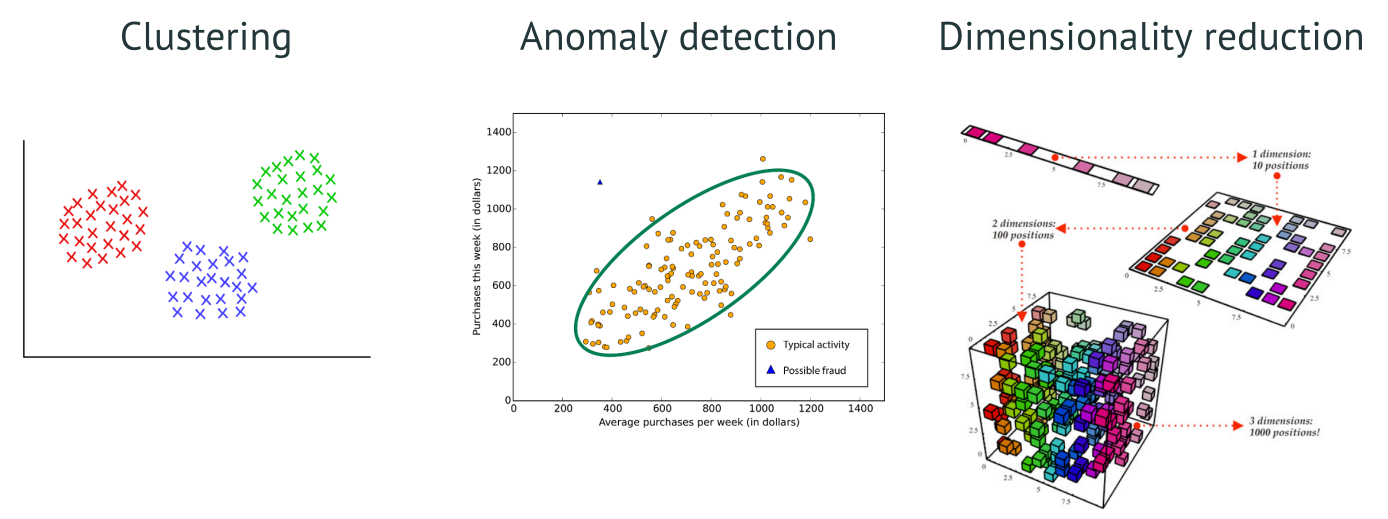
\includegraphics[width=0.7\textwidth]{unsupervised-learning.png}
    \caption{Unsupervised Learning}
\end{figure}

\begin{figure}[H]
    \centering
    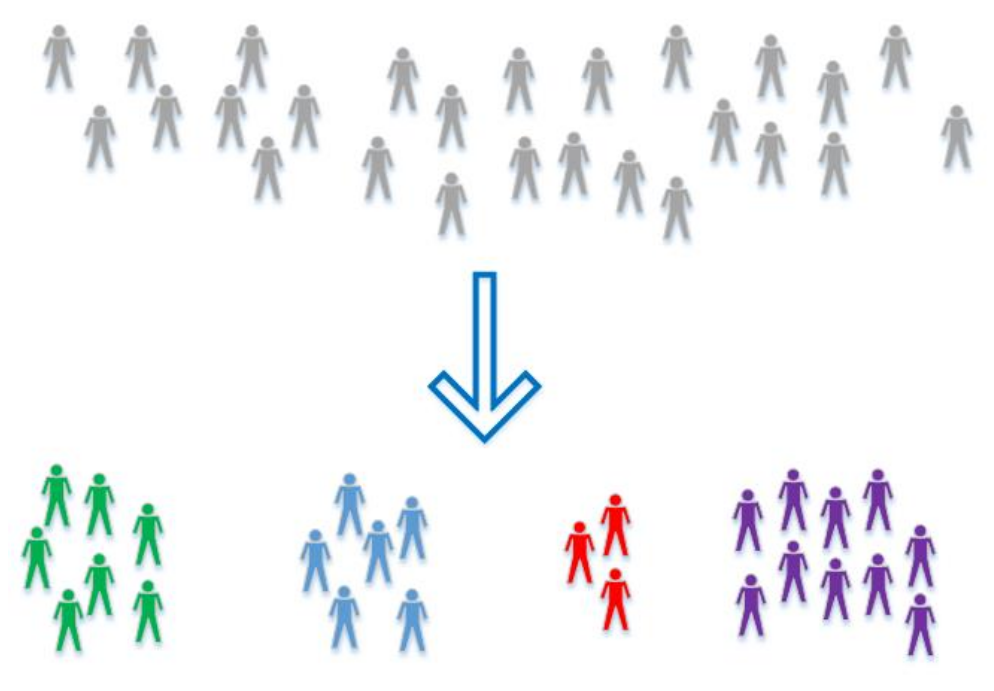
\includegraphics[width=0.5\textwidth]{unsupervised-learning2.png}
    \caption{Voorbeeld Clustering: de data in groepen verdelen}
\end{figure}

\subsection{Reinforcement learning}

\begin{figure}[H]
    \centering
    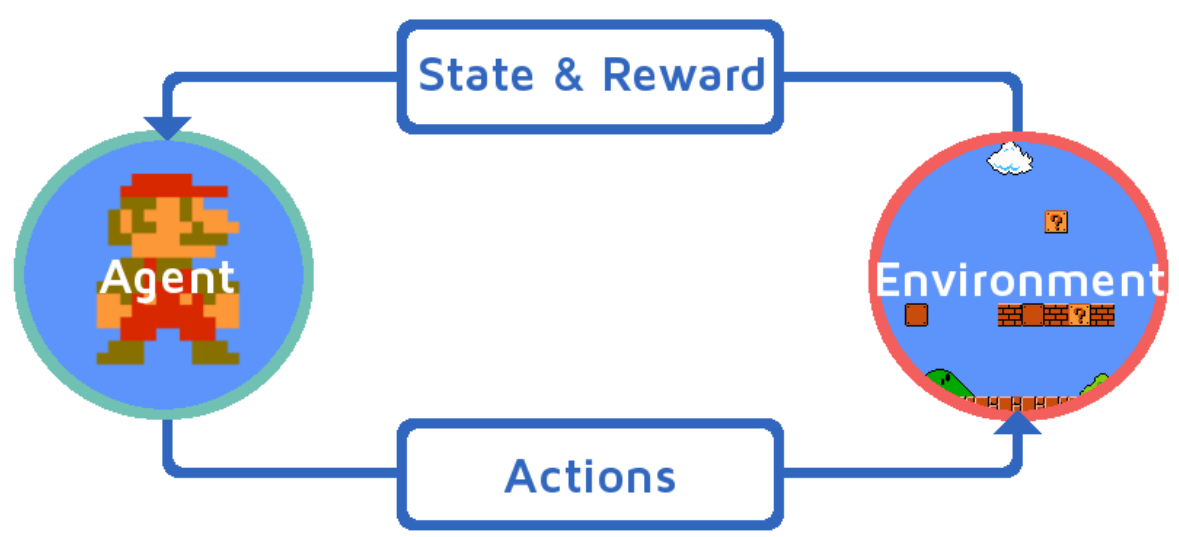
\includegraphics[width=0.5\textwidth]{reinforcement-learning.png}
    \caption{Reinforcement learning}
\end{figure}

\begin{itemize}
    \item Voor elke actie krijgt de AI feedback
    \item De AI leert uit de feedback
    \item In het begin zijn de acties heel willekeurig
\end{itemize}

\subsection{Overzicht leeralgoritmes}

\begin{figure}[H]
    \centering
    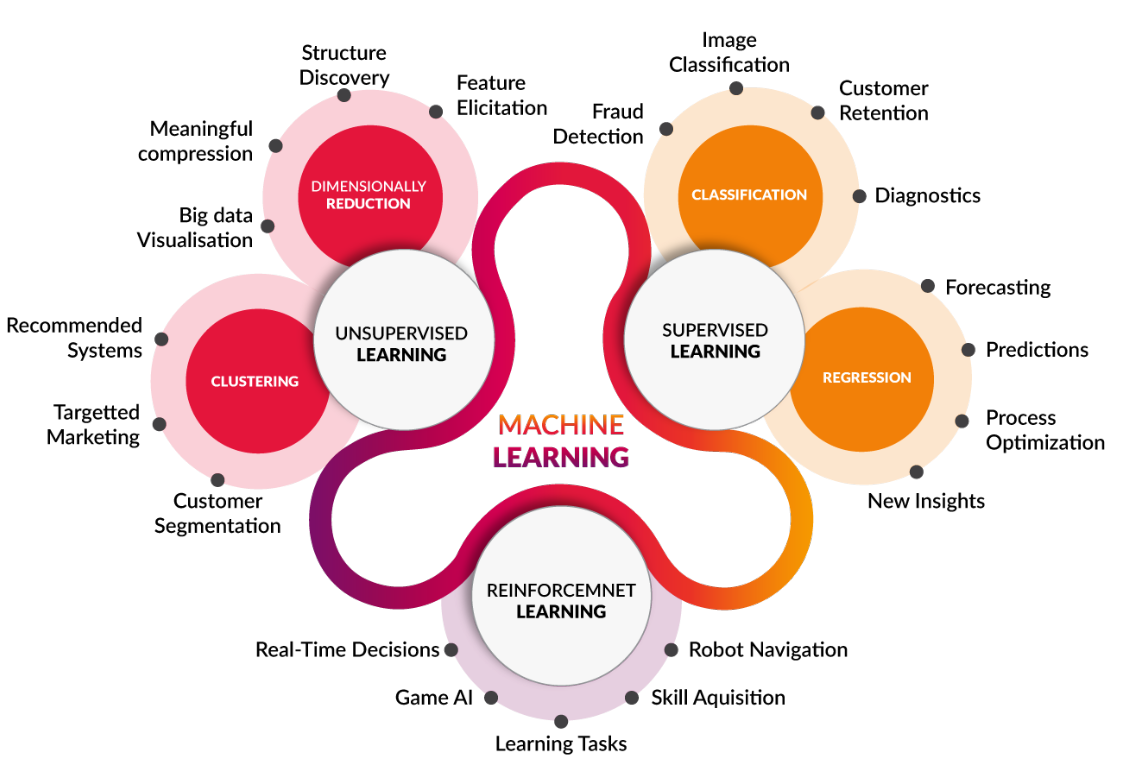
\includegraphics[width=0.55\textwidth]{overzicht-leeralgoritmes.png}
    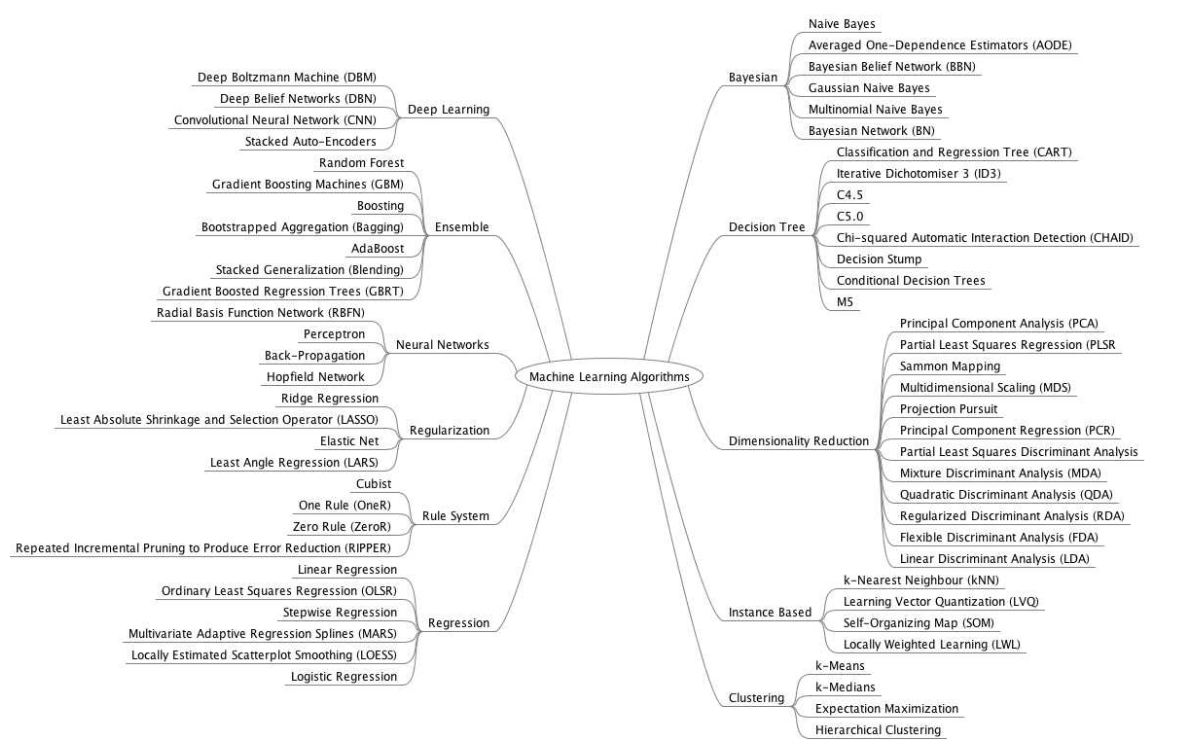
\includegraphics[width=0.5\textwidth]{overzicht-leeralgoritmes2.png}
    \caption{Overzicht}
\end{figure}

\subsection{Werkwijze van een ML Project}

\begin{figure}[H]
    \centering
    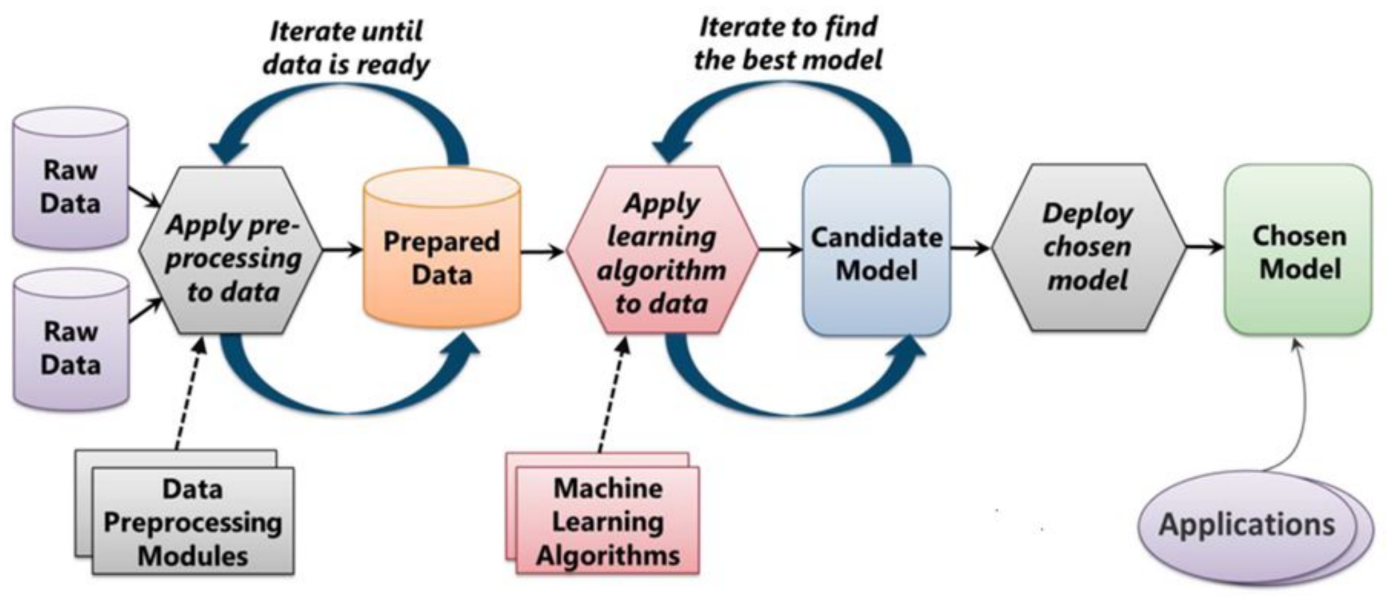
\includegraphics[width=0.4\textwidth]{machine-learning-project.png}
    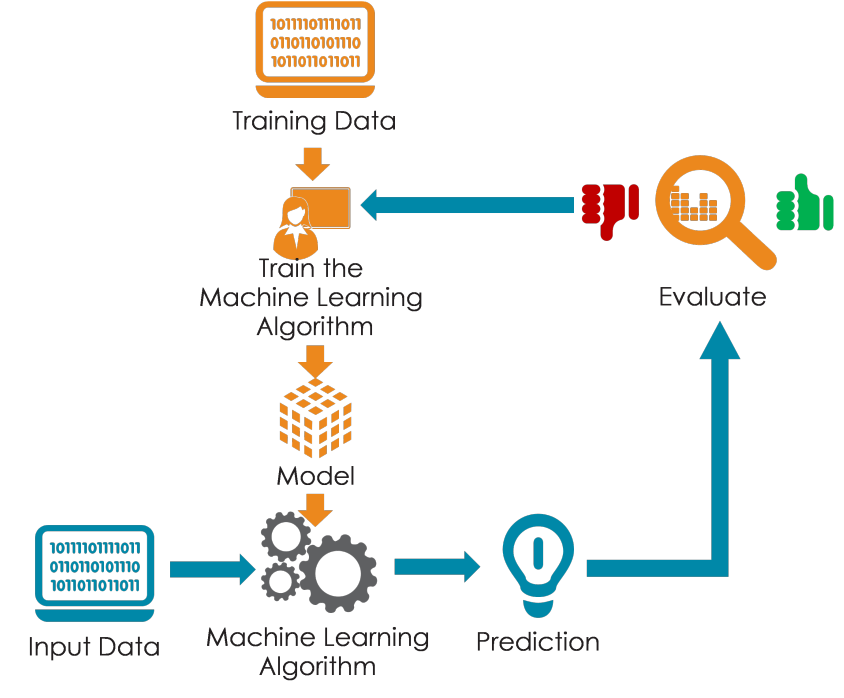
\includegraphics[width=0.35\textwidth]{machine-learning-project2.png}
    \caption{}
\end{figure}

\begin{figure}[H]
    \centering
    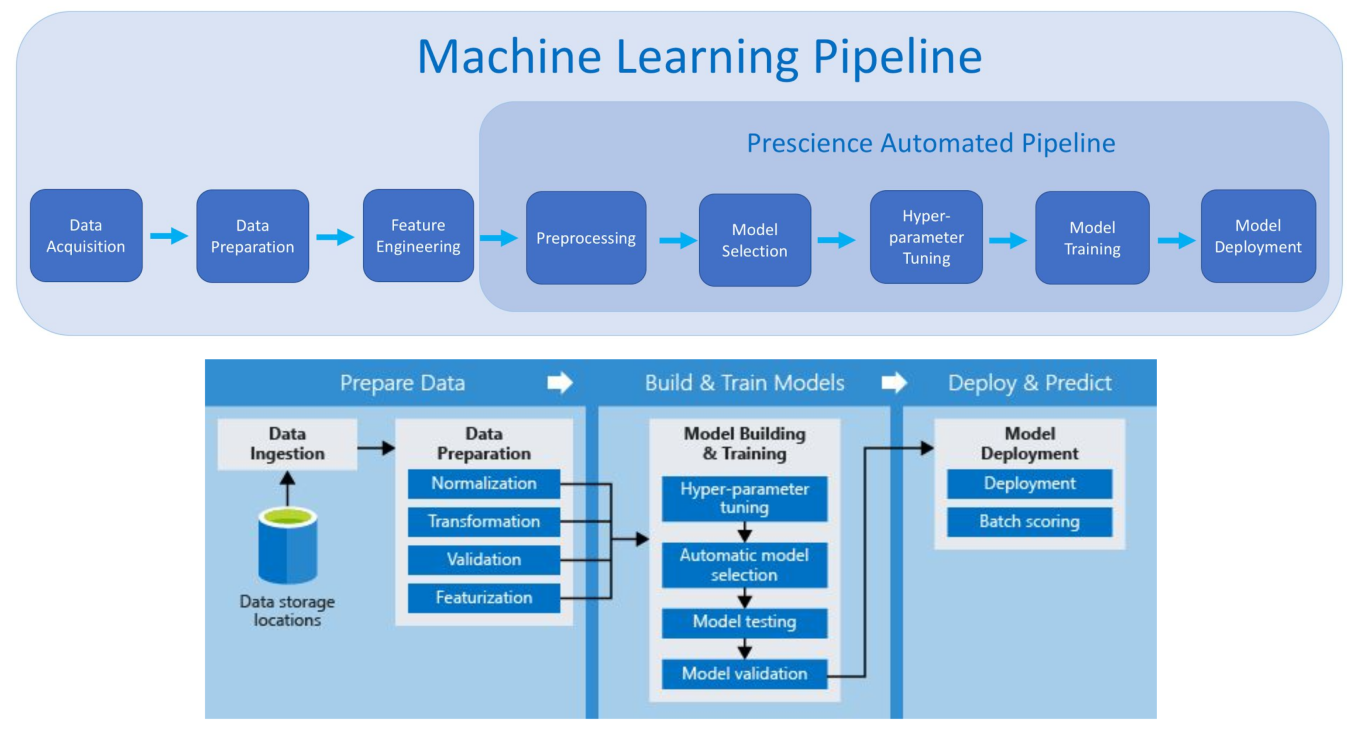
\includegraphics[width=0.45\textwidth]{machine-learning-project3.png}
    \caption{}
\end{figure}

\subsubsection{Tijdverdeling}


\begin{figure}[H]
    \centering
    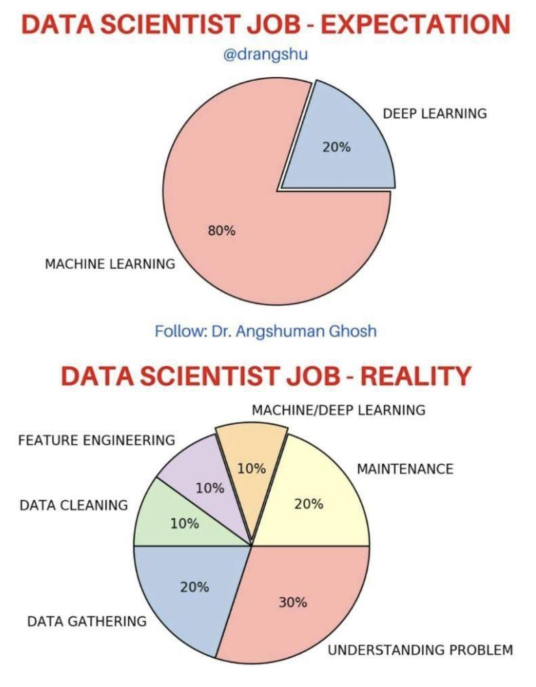
\includegraphics[width=0.35\textwidth]{machine-learning-project4.png}
    \caption{Tijdverdeling: verwachting vs realiteit}
\end{figure}

\section{Enkelvoudige Lineaire regressie}


\end{document}